\documentclass{beamer}
\usepackage{ngerman}
\usepackage{graphicx}
\usepackage{listings}
\usepackage{amsmath}
\usepackage{amssymb}
\usetheme{Madrid}
\title{Algorithmen I Tutorium}
\author{Florian Tobias Schandinat}
\date{09.06.2011}
\institute{FTS}
\lstset{basicstyle=\small\ttfamily,tabsize=4,showstringspaces=false}


\begin{document}


\begin{frame}
\frametitle{Willkommen}
\begin{block}{Algorithmen I Tutorium 19}
\begin{description}
\item[Wer?] Florian Tobias Schandinat\\
\item[Wo?] 50.34, Raum -118\\
\item[Wann?] jeden Donnerstag 15:45-17:15
\end{description}
\end{block}

\begin{block}{Material online}
http://github.com/schandinat/algorithmen1\_ss11
\end{block}
\end{frame}


\begin{frame}
\frametitle{Graphenrepr"asentation}
\begin{exampleblock}{"Ubung}
$V = \{1, 2, 3, 4\}$\\
$E = \{(1, 2), (1, 3), (3, 1), (3, 2)\}$\\

Beschreiben Sie den Graphen $G=(V,E)$ mittels
\begin{itemize}
\item Adjazenzliste
\item Adjazenzmatrix
\item Adjazenzfeld
\end{itemize}

\pause

F"ugen Sie nun die Kante $(2, 4)$ ein
\end{exampleblock}
\end{frame}


\begin{frame}
\frametitle{Graphenrepr"asentation -- "Ubersicht}
\begin{block}{Adjazenzliste}
\begin{itemize}
\item schnelles Hinzuf"ugen von Kanten
\item Speicherverbrauch: $\theta(|V| + |E|)$
\end{itemize}
\end{block}

\begin{block}{Adjazenzmatrix}
\begin{itemize}
\item schnelle Kantenabfrage
\item schnelles Hinzuf"ugen/L"oschen von Kanten
\item Speicherverbrauch: $\theta(|V|^2)$
\end{itemize}
\end{block}

\begin{block}{Adjazenzfeld}
\begin{itemize}
\item etwas kompakter und etwas schnellere Kantenabfrage als Adjazenzliste
\item Hinzuf"ugen/L"oschen von Kanten ist teuer
\item Speicherverbrauch: $\theta(|V| + |E|)$
\end{itemize}
\end{block}
\end{frame}


\begin{frame}
\frametitle{Tiefensuche (DFS)}
\begin{center}
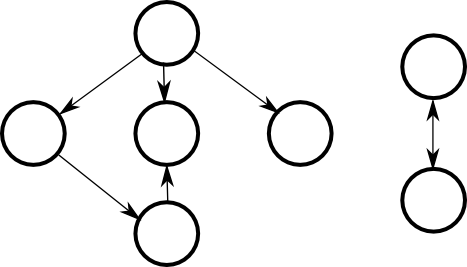
\includegraphics{search_start}
\end{center}
\end{frame}


\begin{frame}
\frametitle{Tiefensuche (DFS)}
\begin{center}
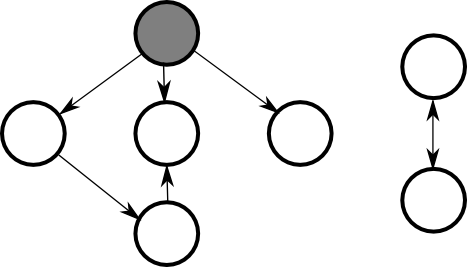
\includegraphics{dfs1}
\end{center}
\end{frame}


\begin{frame}
\frametitle{Tiefensuche (DFS)}
\begin{center}
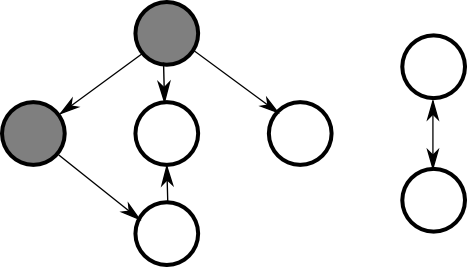
\includegraphics{dfs2}
\end{center}
\end{frame}


\begin{frame}
\frametitle{Tiefensuche (DFS)}
\begin{center}
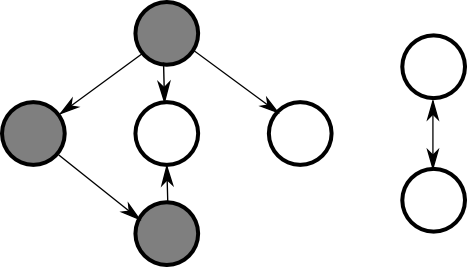
\includegraphics{dfs3}
\end{center}
\end{frame}


\begin{frame}
\frametitle{Tiefensuche (DFS)}
\begin{center}
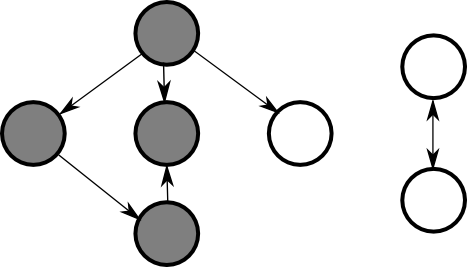
\includegraphics{dfs4}
\end{center}
\end{frame}


\begin{frame}
\frametitle{Tiefensuche (DFS)}
\begin{center}
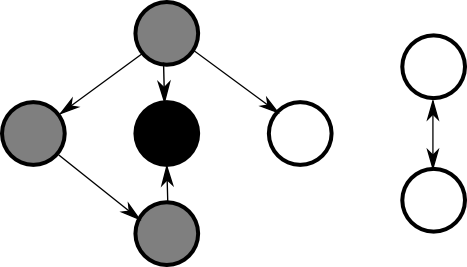
\includegraphics{dfs5}
\end{center}
\end{frame}


\begin{frame}
\frametitle{Tiefensuche (DFS)}
\begin{center}
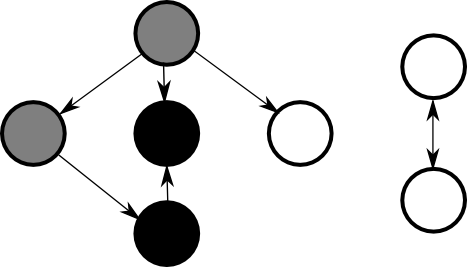
\includegraphics{dfs6}
\end{center}
\end{frame}


\begin{frame}
\frametitle{Tiefensuche (DFS)}
\begin{center}
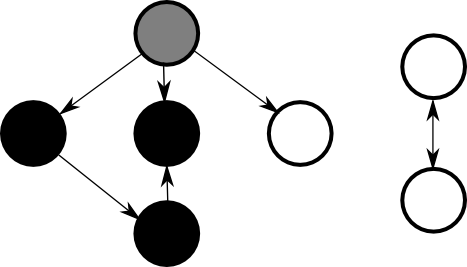
\includegraphics{dfs7}
\end{center}
\end{frame}


\begin{frame}
\frametitle{Tiefensuche (DFS)}
\begin{center}
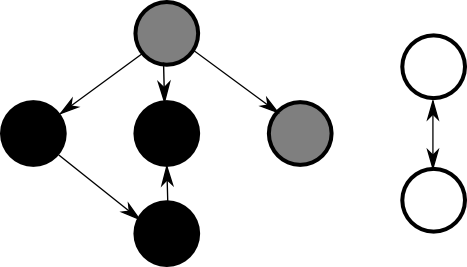
\includegraphics{dfs8}
\end{center}
\end{frame}


\begin{frame}
\frametitle{Tiefensuche (DFS)}
\begin{center}
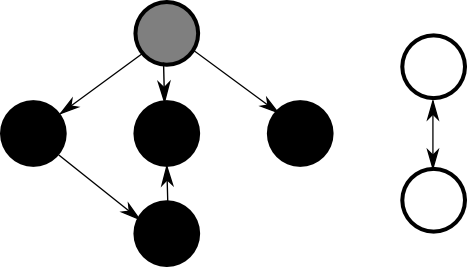
\includegraphics{dfs9}
\end{center}
\end{frame}


\begin{frame}
\frametitle{Tiefensuche (DFS)}
\begin{center}
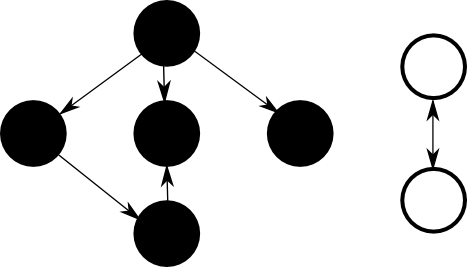
\includegraphics{dfs10}
\end{center}
\end{frame}


\begin{frame}
\frametitle{Tiefensuche (DFS)}
\begin{center}
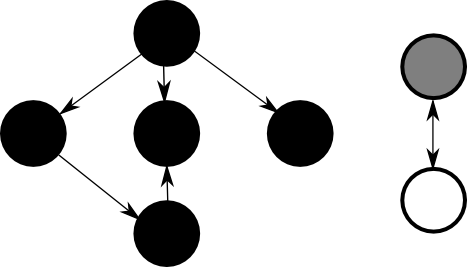
\includegraphics{dfs11}
\end{center}
\end{frame}


\begin{frame}
\frametitle{Tiefensuche (DFS)}
\begin{center}
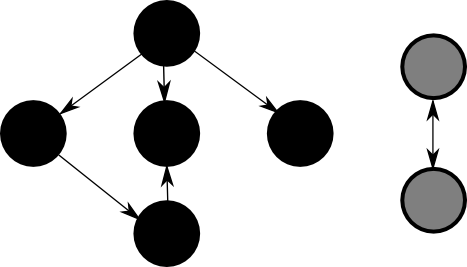
\includegraphics{dfs12}
\end{center}
\end{frame}


\begin{frame}
\frametitle{Tiefensuche (DFS)}
\begin{center}
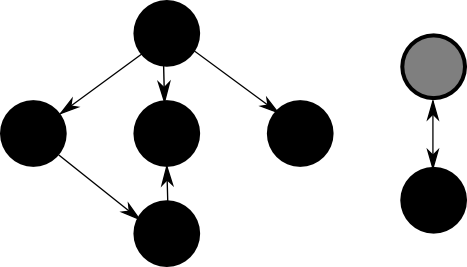
\includegraphics{dfs13}
\end{center}
\end{frame}


\begin{frame}
\frametitle{Tiefensuche (DFS)}
\begin{center}
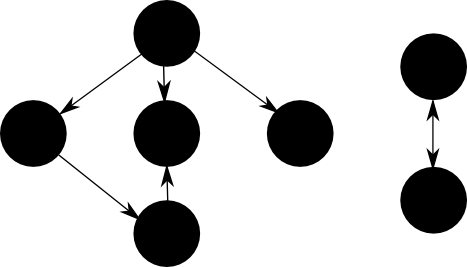
\includegraphics{dfs14}
\end{center}
\end{frame}


\begin{frame}
\frametitle{Breitensuche (BFS)}
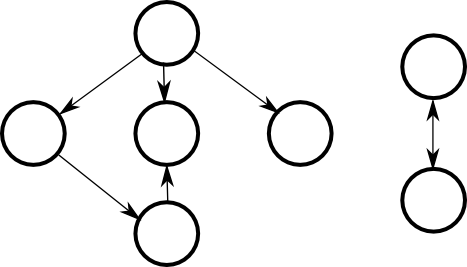
\includegraphics{search_start}
\end{frame}


\begin{frame}
\frametitle{Breitensuche (BFS)}
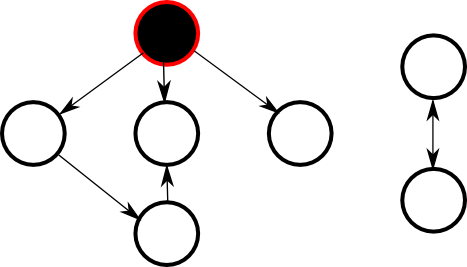
\includegraphics{bfs1}
\end{frame}


\begin{frame}
\frametitle{Breitensuche (BFS)}
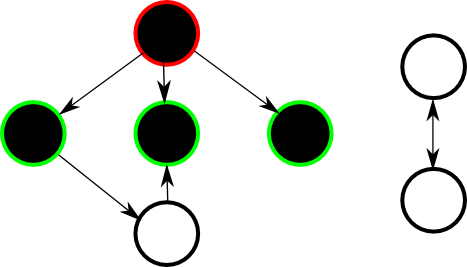
\includegraphics{bfs2}
\end{frame}


\begin{frame}
\frametitle{Breitensuche (BFS)}
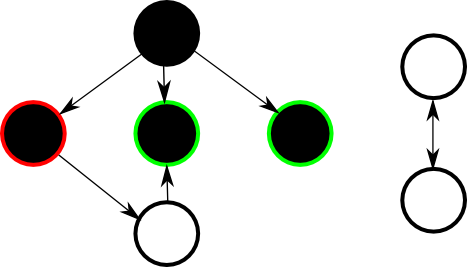
\includegraphics{bfs3}
\end{frame}


\begin{frame}
\frametitle{Breitensuche (BFS)}
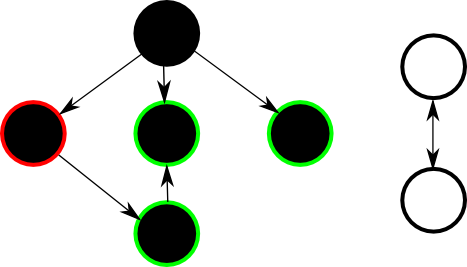
\includegraphics{bfs4}
\end{frame}


\begin{frame}
\frametitle{Breitensuche (BFS)}
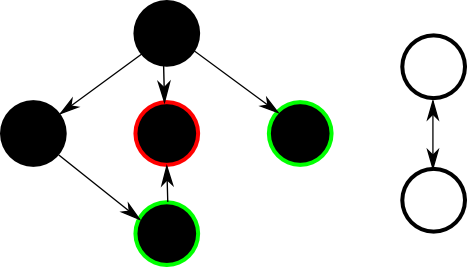
\includegraphics{bfs5}
\end{frame}


\begin{frame}
\frametitle{Breitensuche (BFS)}
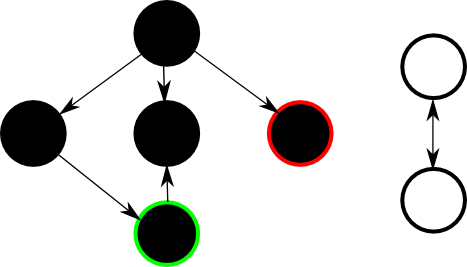
\includegraphics{bfs6}
\end{frame}


\begin{frame}
\frametitle{Breitensuche (BFS)}
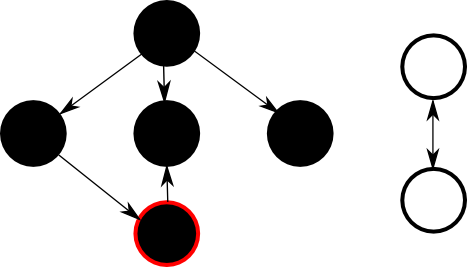
\includegraphics{bfs7}
\end{frame}


\begin{frame}
\frametitle{Breitensuche (BFS)}
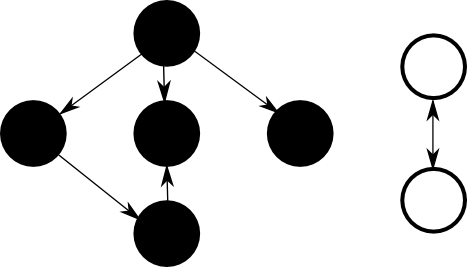
\includegraphics{bfs8}
\end{frame}


\begin{frame}
\frametitle{DFS \& BFS}
\begin{block}{DFS}
\begin{itemize}
\item kein ausgezeichneter Startknoten
\item discovered, finalized
\item Depth-First-Forest
\item Laufzeit: $\theta(|V| + |E|)$
\end{itemize}
\end{block}

\begin{block}{BFS}
\begin{itemize}
\item ausgezeichneter Startknoten
\item distance
\item Breadth-First-Tree
\item Laufzeit: $\theta(|V| + |E|)$
\end{itemize}
\end{block}
\end{frame}


\begin{frame}
\frametitle{Sonstiges}
\begin{block}{}
\begin{itemize}
\item Baumkante
\item R"uckw"artskante
\item Vorw"artskante
\item Querkante
\item Klammern-Theorem
\item Starke Zusammenhangskomponenten
\item Bipartite Graphen
\end{itemize}
\end{block}
\end{frame}


\begin{frame}
\frametitle{Ende}
\begin{center}
\textbf{\Huge Vielen Dank f"ur die Aufmerksamkeit!}
\end{center}
\end{frame}


\end{document}

